\section{ SR03NL12 }


\subsection{Meta}

    \textbf{Title:}
    Taxonomic classification of planning decisions in health care: a structured review of the state of the art in OR/MS

    \begin{table}[H]
        \centering
        \begin{tabular}{|c|c|c|c|c|c|c|c|c|}
            \hline
                \textbf{Rank} & \textbf{Grasp} & \textbf{Grade} & \textbf{Type} & \textbf{Outcome} & \textbf{Domain} & \textbf{COV19} & \textbf{CoI} & \textbf{DB} \\
            \hline
                4 & 94\% & A & A & P & B & No & ?? & No \\
            \hline
        \end{tabular}
        \caption{Reference's metadata}
        \label{tab:SR03NL12}
    \end{table}

\subsection{Summary}
    Peter J. H. et al. produced significant visionary work underlining and defining healthcare services based on the decision-making processes. The authors introduced a taxonomy framework and reviewed more than 400 publications in its scope. This work is outdated regarding the relative methods for a particular healthcare problem. Nevertheless, the value of this research lies in the terminology and classification methodology. After each subsection, the methods available at the time were highlighted. The authors underline five solution domains: computer simulation, Markov processes, math programming, queueing theory, and heuristics. The preset literature review has significant value in establishing a taxonomy structure and describing the existing healthcare problems from the decision-making perspective.
    

\subsection{Notes}
    \begin{itemize}
        \item ORchestra - literature database introduced and maintained by the Center for Healthcare Oprations Improvement and Research (CHOIR);
        \item Definitions of Strategic Planning, Tactical Planning, Operational Planning, Offline OP, and Online OP;
        \item Healthcare services definitions;
        \item Data Envelopment Analysis (DEA) and Stichastic Frontier Analysis (SFA) (91);
        \item Search terms in the Appendix B;
        \item Business Source Elit (135), PubMed (346), and Scopus (372) did not add much literature materials;
        \item Definitions of the healthcare services in the each level of the decision-making hirarchi;
        \item Look into Markov processes;
        \item Valuable Appendices at the end of the paper; 
    \end{itemize}


\subsection{Reading}
    \textbf{Abstract:}
    The authors provide a taxonomy analysis and review of the papers in Operations Research amd Management Science for the Healthcare. The review descrives the existing techniques (prior 2012) for making a planning and controll desicions.
    
    \textbf{Objectives:}
    Aim to guide healthcare proffectionals in the field of OR/ MS.

    
    \textbf{Page 1:}
    The first page provides a basic introduction into the field of effective resource management. The definition of the Operations Research and Management Science as a cross field of various natural and cosial scinces. 
    
    \textbf{Page 2:}
    The authours touched on the application of the OR/MS and also introduces the CHOIR and ORchestra database. The paper contains sections dedicated taxomony, OR/ MS practicies in healthcare, and the literature review. The authors layed out the deeper explanation of the taxonomy and explaned the architecture of the healthcare services by level of desicion making (strategic, tactical, opearional-offline, operational-online).
    
    \textbf{Page 3:}
    More about selected taxonomy approach. Here are presented definitions for each of the desicion-making levels.
    \begin{figure}[H]
        \centering
        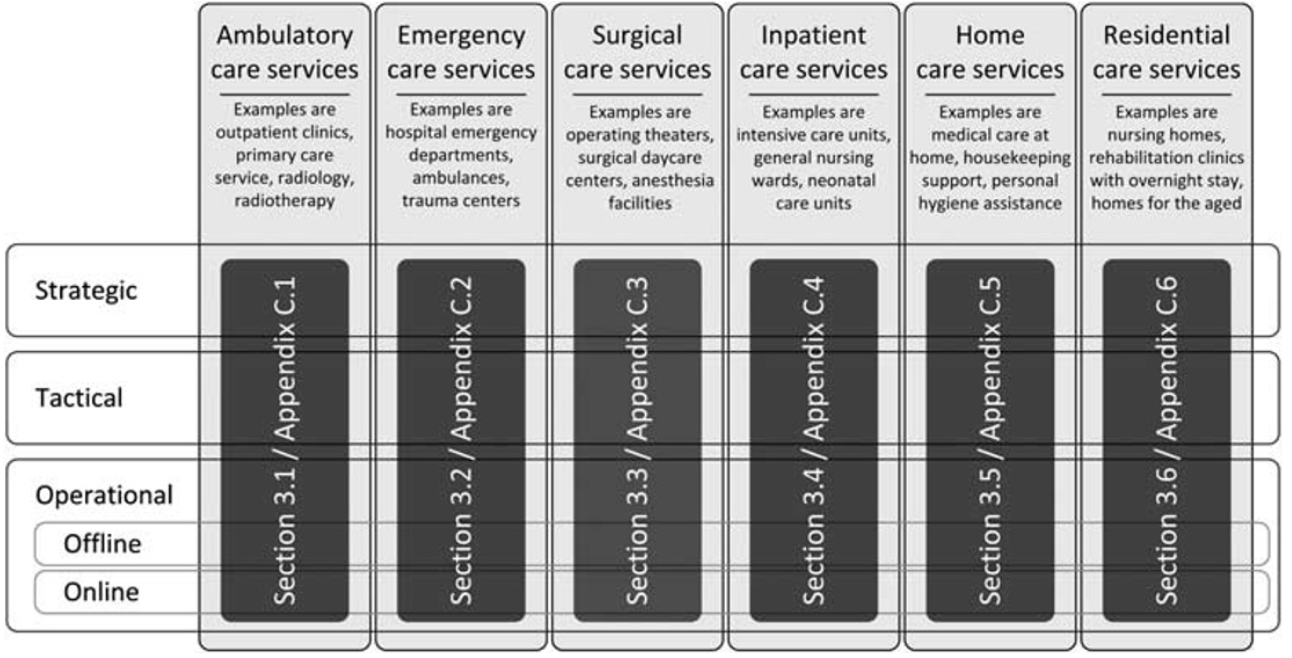
\includegraphics[width=1\textwidth]{figures/0011_SR03NL12/fig1.png}
        \caption{Visualisation of the OR/MS structure in healthcare \cite{x029}.}
        \label{fig1:0011_SR03NL12}
    \end{figure}

    \textbf{Page 4:}
    The interconnections between the desicion-making levels are outlined on this page. Then the definisions for multiple healthcare services are presented.

    \textbf{Page 5:}
    The research questions, methodology, and the methods were described in more details. The authors ephacise the need to focus on decision-making aspects of healthcare.
    \begin{figure}[H]
        \centering
        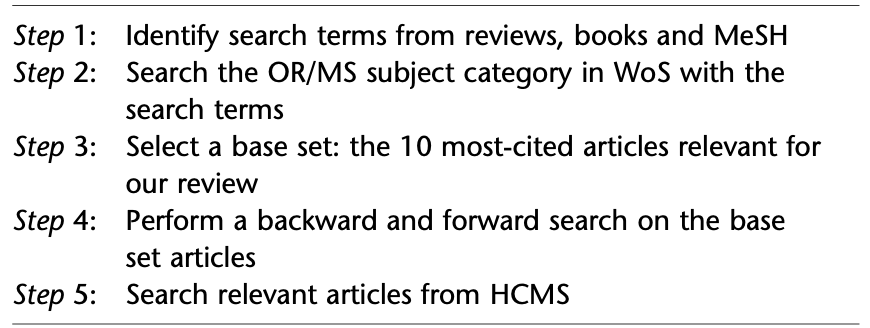
\includegraphics[width=1\textwidth]{figures/0011_SR03NL12/fig2.png}
        \caption{The search method applied for each healthcare service in \cite{x029}.}
        \label{fig2:0011_SR03NL12}
    \end{figure}
    
    \textbf{Page 6:}
    More healthcare services' definitions. \underline{Regional coverage} = Ambulance care + location + demand (methods: si,ulation, heuristics, has lit. review). \underline(Service mix) = organisation decision + ambulatory service (methods: no papers found). \underline{Case mix} = facility + patient group (methods: not much but simulation, and math programming). \underline{Panel size} = demand and capacity balance (methods: simulation, queueing theory). \underline{Capacity dimansioning} = consultaiont room + staff + consultation time capacity + equipment + waiting room (methods: simulation, Markov processes, math programming, queueing theory, lit. review)...
    
    \textbf{Page 7:}
    ...\underline{Facility layout} = reception area + waiting area + conculstaion room (methods: no articles, but there is a book on heuristics). \underline{Patient routing} = flow + optimization(methods: simulation, queueing theory). \underline{Capacity allocation} = resource group + patient group + time subdivision (simulation, math models, lit. review). \underline{Temporary capacity change} = equilibrium between time access and utilisation (methods: simulation). \underline{Access policy} = healthcare accessability + appointment type (walk-in, same-day, standart schedule; methods: simulation, heuristic, Markov processes, queueing theory)...
    
    \textbf{Page 8:}
    ... \underline{Adminssion control} = waiting list + rules of access (methods: simulation, heuristics, Markov processes, math. programming). \underline{Appointment scheduling}: Number of patients per consultation, Patient overbooking, Length of the appointment intercal, Number of patients per appointment slot, Sequence of appointment, Queue discipline in the waiting room, Anticipation for inscheduled patients (methods: simulation, heuristics, Markov processes, math programming, queueing theory, lit. review)... 
    
    \textbf{Page 9:}
    ... \underline{Staff-shift scheduling} = staff + timetable + demand-capacity balance (methods: simulation, math programming, lit. review). | Offline operational planning |: \underline{patient-to-appointment assignment} = appointment time + facility + patient, examples are: Signle appointment, Combination appointment, Appointment series (methods: heuristics, Markov processes, math programming). \underline{Staff-to-shift assignment} = medical personnel + timetable (methods: meth programming, lit. review). | Online operational planning | \underline{Dynamic Patient (re)assignment} = uncertainties + patient + rescheduling (methods: simulation, Markov processes, math programming). \underline{Staff rescheduling} = demand fluctuations + staff absenteeism (no paper found).
    
    \textbf{Page 10:}
    This page underlines the \underline{Emergency care services} particularly by their regional coverage. This includes the location of the emergency care centers and the available trasportation in ambulance to reach far regions (methods: simulation, heuristics, Merkov processes, mathematical programming, lit. review)\dots
    
    \textbf{Page 11:}
    ... \underline{Service mix} = services + emergency (methods: no papers found). \underline{Ambulance districting} = area segmentation + ambulance (methods: simulation, heuristics, mathematical programming, queueing theory).\underline{Copacity dimensioning} = emergency + facility capacity + minimal costs + availability (methods: simulation, heuristics, math programming, queueing theory, lit. review)...
    
    \textbf{Page 12:}
    ...\underline{Facility layout} as the name suggests (methods: simulation, heuristic, lit. review). | Tactical planning | \underline{Patient routing} = emergency + patient flow + desicion-making (methods: simulation, queueing theory, lit. review). \underline{Admission control} = priorities + demand-capacity balabce (methods: simulation, queueing theory). \underline{Staff-shift scheduling} = demand-capacity balance + medical personnel (methods: simulation, heuristics, queueing theory, lit. review)...
    
    \textbf{Page 13:}
    ...| Offline Operational Planning | \underline{staff-to-shift assignment} = minimise costs + personnel availability (methods: heuristics, math programming). | Online Operational Planning | \underline{ambulance dispatching} = emergency + logistics + priority (methods: simulation, heuristics, math. programming, queueing theory). \underline{facility selection} = logistics + priority (methods: simulation). \underline{Ambulance routing} = logistics (methods: no paper found). \underline{Ambulance relocation} = logistics + desicion-making (methods: simulation, Markov processes, math programming, lit. rev)...
    
    \textbf{Page 14:}
    ... \underline{Treatemtn planning and prioritization} = prescriptions + urgency + medical resource availability, also ~facility layout, ~patient routing, and ~admission control (methods: simulation). \underline{Staff rescheduling} = capacity flexibility + staff availability (methods: simulation, math. programming). | SURGICAL CARE SERVICES - Strategic Planning | \underline{Regional coverage} = facility prioritisation (methods: simulation, math programming). \underline{Service mix} = service prioritisation + demand (methods: no papers found). \underline{Case mix} = patient groups + financial status balance (methods: simulation, math programming, lit. review)...
    
    \textbf{Page 15:}
    ...\underline{Capacity dimensioning} = operating rooms + operating time capacity + presurgical rooms + recovery wards + ambulatory surgical ward + equipment + staff (methods: simulation, heuristics, math programming, queueing theory, lit. review). \underline{facility layout} = demand-capacity balance + location (methods: simulation, heuristics + lit. review).| Tactical Planning | \underline{Patient routing} = pre-, peri-, post-operative rooms (methods: simulation, heuristics, math. programming, lit. review). \underline{Capacity allocation} = patient group identification + time subdivision + block scheduling , and also ~strategic level of patients groups (methods: simulation, heuristics, Markov processes, math programming, lit. review)...

    \textbf{Page 16:}
    ... \underline{Temporary capacity change} = flexible capacity (methods: simulation, math programming, lit. review). \underline{Unused calaptity (re)location} = flexible scheduling (simulation, heuristics, Markov processes, lit. review). \underline{Admission control} = balancing patient services, resource utilsation, and staff satisfaction (methods: simulation, markov processes, math programmin, lit. review)...

    \textbf{Page 17:}
    ... \underline{Staff-shift scheduling} = capacity-demand balancing (methods: heuristic, meth programming, lit. review). | Offline operational planning | \underline{Staff-to-shift assignment} = dinamic scheduling (methods: no papers found). \underline{Surgical case scheduling} = preoperative stage duration + surgical procedure duration + switching time + postsurgical recovery duration + emergency patient interruption + staff availability + starting time of a surgery (methods: simulation, heuristics, Markov processes, math programming, queuering theory, lit. review)\dots
    
    \textbf{Page 18:}
    ... | Online operational planning | \underline{Emeregency case scheduling} = prioritisation + rescheduling + flexible scheduling (methods: math programming, lit. review). \underline{Surgical case rescheduling} = rescheduling + flexible scheduling (methods: math programming, lit. review). \underline{Staff rescheduling} = ?? (methods: no paper found). | INPATIENT CARE SERVICES - Strategic planning | \underline{regional coverage} = facilities' number + type + location (methods: simulation, math programming, queueing theory)...

    \textbf{Page 19:}
    ... \underline{Service mix} = hospital facilities (methods: no papers found). \underline{Case mix} = capacities for patients (methods: simulations, heuristics). \underline{Case unit partitioning} = healthcare department segmentation (methids: simulation, meth programming, queueing theory)... 
    
    \textbf{Page 19:}
    ...\underline{Capacity dimensioning} = beds + euqipment + staff (methods: simulation, heuristics, Markov processes, math programming, queueing theory, lit. review)... 
    
    \textbf{Page 20:}
    ... \underline{Facility layout} = flexible/ modular space (methods: si,ulation, heuristic, math programming). | Tactical Planning | \underline{Bed reallocation} = prioritisation of the capacity (methods: simulation, heuristics, math programming, queueing theory). \underline{Temporary bed copacity change} = trends/ season prediction (methods: simulation, heuristics, queueing theory). \underline{Admission control} = time management, which can be static or dynamic, also static/ dynamic bed reservation, overflow rules, influence surgical schedule (methods: simulation, heuristics, Markov processes, math programming, queueing theory)...
    
    \textbf{Page 21:}
    ... \underline{Staff-shift scheduling} = demand prediction + capacity allocation + inpatient (methods: simulation, heuristics, math programming, queuering theory, lit. review). | Offline Operational Planning | \underline{Admission scheduling} = rules for patient time and service allocation (math programming). \underline{Patient-to-bed assignment} = patient preferences + availability (methods: heuristics, math programming). \underline{Discharge planning} = discharge rules and regulations aimed to reduce "bed blocking" (methods: simulation, queueing theory, lit. review)...
    
    \textbf{Page 22:}
    ... \underline{Staff-to-shift assignment} = several weeks + shift assingment (methods: heuristics, math programming, lit. review). | Online operational planning | \underline{Elective admission rescheduling} = desicion macking + flexible scheduling (methods: simulation, heuristics, queueing theory). \underline (Acure admission handling) = admision rules + desicion-macking (methods: simulation, queueing theory). \underline{Staff schedulign} = personnel availabitili, also consider float, part-time, on-call, absenteesim, and voluntary shifts (methods: simulation, math programming, lit. review). \underline{Nurse-to-patient assignment} = allocating patient care + workload balance (methods: simulation, heuristics, math programming). \underline{Transfer scheduling} = staff choriography (methods: Markov processes). 
    
    \textbf{Page 23:}
    | HOME CARE SERVICES - Strategic Planning | \underline{Placement policy} = patient groups + elligability rules (methods: heuristics, Markov processes, math programming, lit. review). \underline{Reglonal coverage} = care capacity + location (methods: lit. review). \underline{Service mix} = service group selection (methods: lit. review). \underline{Case mix} = service selection + demand (methods: lit. review). \underline{Panel size} = demand forcasting + planning (methods: math programming)... 
    
    \textbf{Page 24:}
    ... \underline{Districting} = logistics + demand evaluation (methods: heuristics, lit. review). \underline{Capacity dimensioning} = resource availability such as staff, equipment, fleet vehicles + budget planning + bottlenetck management (methods: simulation, Markov processes, queueing, lit. review). | Tactical planning | \underline{Capacity allocation} = considering areas and patient groups + workload balance (methods: heuristics, math programming, queueing theory, lit. review). \underline{Admission control} = demand-supply balance + demand evaluation (methods: Markov processes, math programming, queueing theory)... 
    
    \textbf{Page 25:}
    ... \underline{Staff-shift scheduling} = uncertainties + patient preferences + personnel availability (methods: heuristics, lit. review). | Offline Operational Planning | \underline{Assessment and intake} = patient elligability (methods: heuristics, Markov ptocesses, math programming, lit. review). \underline{Staff-to-shift assingment} = personnel assignemnt for several weeks ahead (methods: heuristics, math programming, lit. review)...
    
    \textbf{Page 26:}
    ... \underline{Visit scheduling} = short-term plan + staff-to-visit assignment + route creation (methods: heuristics, Markov processes, mathematical programming, lit. review). | Online Operational Planning | \underline{Visit reschediling} = emergency perception + flex scheduling (methods: heuristics, mathematical programming). \underline{Residential case services} = governments + rules and regulations. | Strategic Planning | \underline{Placement policy} = rules and regulations + capacity planning + patient evaluation (methods: simulation, heuristics, Markov processes, queueing theory)... 
    
    \textbf{Page 27:}
    ... \underline{Regional coverage} = logistics + patient evaluation + capacity planning (methods: math programming, lit. review). \underline{Case mix} = patient classification, for instance rehabilitation short-stay or a geriatric long-stay (methods: heuristics). \underline{Capacity dimenshioning} = facilities + equipment + personnel (methods: conputer simulation, Markov processes, queueing theory). 
    
    \textbf{Page 28:}
    | Tactical Planning | \underline{Admission control} = rules and guidance + priority (methods: simulation, math programming). | Offline Operational Planning | \underline{Treatment scheduling} = weeks in advances + patient evaluation + demand evaluation (methods: math programming).
    
    \textbf{Conclusion:}
    The authors dedicated this research to healthcare proffesionals to increase their awairness and to improve the healthcare scheduling practicies. In the review the taxonomy framework was introduces and the literature analysis was carried on followith the structure of the framework. The authors claimed that the desicion-making in healthcare has promising results now and further potential for the future research.
    